% !TEX TS-program = pdflatex
% !TEX encoding = UTF-8 Unicode

% This file is a template using the "beamer" package to create slides for a talk or presentation
% - Talk at a conference/colloquium.
% - Talk length is about 20min.
% - Style is ornate.

\documentclass{beamer}

\mode<presentation>
{
  \usetheme{Marburg}
  \setbeamercovered{transparent}
  % or whatever (possibly just delete it)
}


\usepackage[english]{babel}
\usepackage[utf8]{inputenc}

%\usepackage{times}
%\usepackage[T1]{fontenc}
% Or whatever. Note that the encoding and the font should match. If T1
% does not look nice, try deleting the line with the fontenc.

%NB: gebruik \dops{} of \dops~ om netjes een whitespace erachter te krijgen in lopende tekst
\newcommand{\dops}[0]{DOP$ ^*$}
\newcommand{\ddop}[0]{Double-DOP}

\newcommand{\pijl}[0]{$\rightarrow$}

%figures:
\usepackage{tikz}
\usetikzlibrary{trees,positioning,backgrounds}
\usetikzlibrary{shapes.multipart}
\usepackage{tikz-qtree}


\title{Doubling \dops}
\subtitle{ A comparison of \ddop{} and \dops{}}
\author[Kruit, Veldhoen]{Benno Kruit\and Sara Veldhoen{\\\vspace{.6cm}\small Supervised by: \\Andreas van Cranenburg \and Khalil Sima'an}}

\institute{University of Amsterdam (UvA)}
\date{Project AI, January 2014}



% Delete this, if you do not want the table of contents to pop up at
% the beginning of each subsection:
\AtBeginSubsection[]
{
  \begin{frame}<beamer>{Outline}
    \tableofcontents[currentsection,currentsubsection]
  \end{frame}
}


% If you wish to uncover everything in a step-wise fashion, uncomment the following command: 
%\beamerdefaultoverlayspecification{<+->}


\begin{document}

\begin{frame}
  \titlepage
\end{frame}

\begin{frame}{Outline}
  \tableofcontents   %[pausesections]
\end{frame}

\section{Data Oriented Parsing}

\subsection{Introduction to DOP}

\begin{frame}{Parsing}%{Subtitle}
  % - A title should summarize the slide in an understandable fashion
  %   for anyone how does not follow everything on the slide itself.

  \begin{itemize}
  \item input: sentence 
\begin{quotation} John Loves Mary \end{quotation}
\pause
  \item output: constituent tree
\begin{figure}
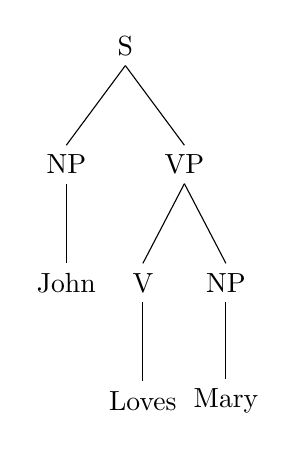
\begin{tikzpicture}
%[node distance = 0 pt, sibling distance=40pt, level distance=40pt,level 2/.style={sibling distance=9pt},level 3/.style={sibling distance=9pt}]
[level 2/.style={sibling distance = 30 pt}]

\node (S) {S}
child { node {NP}  
	child{ node {John}}
	}
child { node {VP} 
	child{ node {V} 
		child {node {Loves}}
		} 
	child{node {NP}
		child {node {Mary}}
		}
	}
;
\end{tikzpicture}

\end{figure}
  \end{itemize}
\end{frame}

\begin{frame}{Grammar}
A grammar describes:
\begin{itemize}
\item how trees can be built
\begin{itemize} 
\item CFG's - elementary rules
\item TSG's  - larger units: \emph{fragments}
\end{itemize}
\item how likely constructions are: \emph{probabilistic} grammars
\begin{itemize} 
\item PCFG's - independence 
\item PTSG's  - derivations
\end{itemize}

\end{itemize}
\end{frame}

\begin{frame}{Grammar: CFG rules}
\begin{quotation}
S\pijl{} NP VP\\
VP\pijl{} V NP\\
NP \pijl{} John\\
NP\pijl{} Mary\\
V\pijl{} loves
\end{quotation}

\end{frame}
\begin{frame}{Grammar: Tree fragments}

\begin{figure}
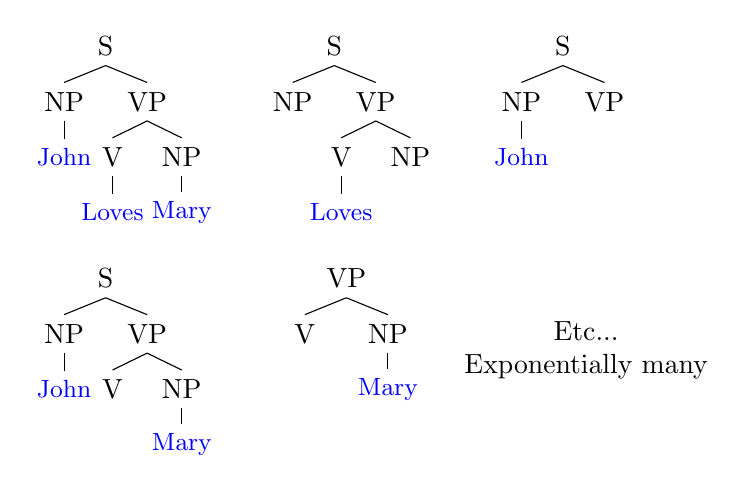
\begin{tikzpicture}
[node distance = 70 pt, sibling distance=30pt, level distance=20pt,level 2/.style={sibling distance=25pt},level 3/.style={sibling distance=15pt}]
%[level 2/.style={sibling distance = 30 pt}]

\node (f1) {S}
child { node {NP}  
	child{ node [color=blue]{\small John}}
	}
child { node {VP} 
	child{ node {V} 
		child {node [color=blue]{\small Loves}}
		} 
	child{node {NP}
		child {node [color=blue]{\small Mary}}
		}
	};
\node (f2)[right=of f1] {S}
child { node {NP} 
	}
child { node {VP} 
	child{ node {V} 
		child {node [color=blue]{\small Loves}}
		} 
	child{node {NP}
		}
	};
\node (f3)[right=of f2] {S}
child { node {NP}  
	child{ node [color=blue]{\small John}}
	}
child { node {VP} 
	};

\node (f4)[below=of f1] {S}
child { node {NP}  
	child{ node [color=blue]{\small John}}
	}
child { node {VP} 
	child{ node {V} 
		} 
	child{node {NP}
		child {node [color=blue]{\small Mary}}
		}
	};

\node (f5)[right=of f4] {VP} 
	child{ node {V} 
		} 
	child{node {NP}
		child {node [color=blue]{\small Mary}}
		};
\node(etc)[below right = 0cm and 1cm of f5, align=center]{\\Etc...\\ Exponentially many};
\end{tikzpicture}

\end{figure}


\end{frame}
\subsection{Bias and Consistency}

\begin{frame}{Consistency}

\begin{itemize}
\item Assumption
  \begin{itemize}
  \item Language is an infinite parse tree distribution
  \item Treebank is a finite sample
  \end{itemize}
\\
\item \emph{Estimate} the true distribution
\item Expected estimation should improve when the treebank grows 
$\rightarrow$ expected \emph{loss} should decline
\item {\bf Consistency}: Expected loss becomes 0 when the sample size approaches $\infty$
\end{itemize}
\end{frame}


\begin{frame}{Bias}

\begin{itemize}
\item Assumption
  \begin{itemize}
  \item An estimator should approach \emph{any} distribution
  \item Even finite distributions!
  \end{itemize}
\\
\item If there's a distribution that doesn't match its expected estimate, the estimator is {\bf biased}.
\item What about unseen data?
\item Bias is {\bf good}
\end{itemize}
\end{frame}

\section{\ddop{} and \dops{}: a comparison}

\subsection{Introduction to \ddop{} and \dops{}}
\begin{frame}{\ddop{}}
\begin{itemize}
\item Extraction: Maximal Overlap
\item Estimation: relative frequency 
\item Coverage: PCFG rules
\end{itemize}
\end{frame}

\begin{frame}{\dops{}}
\begin{itemize}
\item Held-out estimation - $HC$ and $EC$
\item Extraction: Shortest derivations
\item Estimation: relative frequency \emph{in shortest derivations}
\item Coverage: smoothing PCFG rules with probability $p_{unkn}$
\end{itemize}
\end{frame}

\subsection{Comparison}
\begin{frame}{Comparison}
\begin{itemize}
\item Shortest derivations or Maximal overlap
\item Split or full estimation
\item Consistency
\end{itemize}
\end{frame}

\begin{frame}{Example}
\begin{figure}
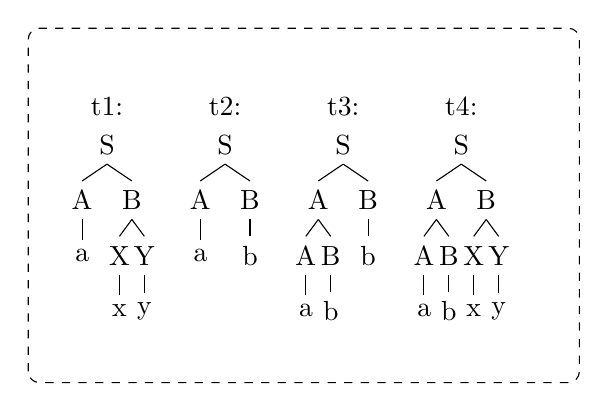
\begin{tikzpicture}
[node distance = 0 pt, sibling distance=18pt, level distance=20pt,level 2/.style={sibling distance=9pt},level 3/.style={sibling distance=9pt}]

\draw[black,dashed,join=round, inner frame sep=2cm and 2cm, rounded corners ] (0,5.5) rectangle (7,10);
%\node[fill = white, rectangle, draw] (treebank) at(2,10) {Treebank};

\node (t1) at(1,9){t1:}
node [ below =of t1] {S}
child {node {A} 	child {node {a}}
	}
child {node {B}	child{node {X}	child{node {x}}}
			child{node {Y}	child{node {y}}}
	}
;

\node (t2) at(2.5,9){t2:}
node [ below =of t2] {S}
child {node {A} 	child {node {a}}
	}
child {node {B}	child{node {b}}
	}
;

\node (t3)  at(4,9){t3:}
node [ below =of t3] {S}
child {node {A} 	child{node {A}	child{node {a}}}
			child{node {B}	child{node {b}}}
	}
child {node {B}	child{node {b}}
	}
; 

\node (t4) at(5.5,9) {t4:}
node [ below =of t4] {S}
child {node {A} 	child{node {A}	child{node {a}}}
			child{node {B}	child{node {b}}}
	}
child {node {B}	child{node {X}	child{node {x}}}
			child{node {Y}	child{node {y}}}
	}
;
\end{tikzpicture}

\caption{A toy treebank}
\end{figure}
\end{frame}

\begin{frame}{Example}
\begin{figure}

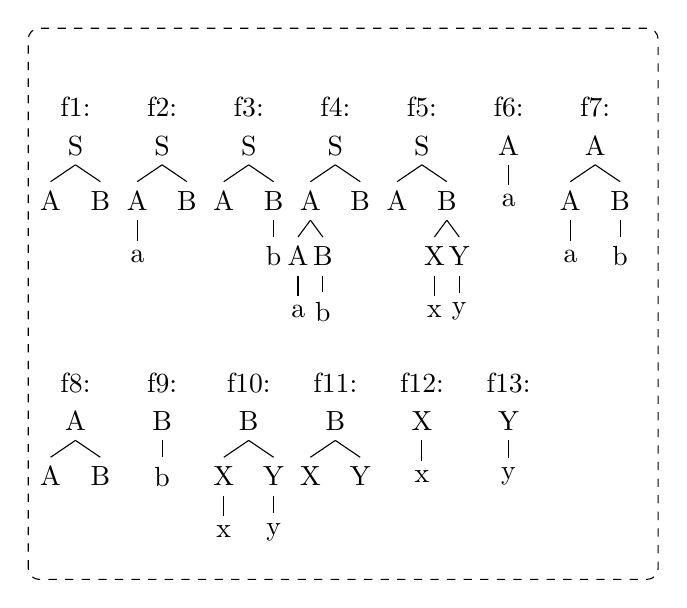
\begin{tikzpicture}
[node distance = 0 pt, sibling distance=18pt, level distance=20pt,level 2/.style={sibling distance=9pt},level 3/.style={sibling distance=9pt}]

\draw[black,dashed,join=round, inner frame sep=2cm and 2cm, rounded corners ] (0,3) rectangle (8,10);
%\node[fill = white, rectangle, draw] (treebank) at(3.5,10) {Fragments with non-zero weights};


\node (f1) at(0.6,9){f1:}
node [ below =of f1] {S}
child {node {A} 		}
child {node {B}		}
;


\node (f2) at(1.7,9){f2:}
node [ below =of f2] {S}
child {node {A} 	child {node {a}}
	}
child {node {B}	}
;

\node (f3)  at(2.8,9){f3:}
node [ below =of f3] {S}
child {node {A} 	}
child {node {B}	child{node {b}}
	}
;

\node (f4) at(3.9,9) {f4:}
node [ below =of f4] {S}
child {node {A} 	child{node {A}	child{node {a}}}
			child{node {B}	child{node {b}}}
	}
child {node {B}		}
;

\node (f5) at(5.0,9) {f5:}
node [ below =of f5] {S}
child {node {A} 		}
child {node {B}	child{node {X}	child{node {x}}}
			child{node {Y}	child{node {y}}}
	}
;

\node(f6) at(6.1,9) {f6:}
node [ below =of f6] {A}	
	child {node {a}}
;

\node(f7) at(7.2,9) {f7:}
node [ below =of f7]  {A} 	
	child{node {A}	child{node {a}}}
	child{node {B}	child{node {b}}}
;




\node(f8) at(0.6,5.5){f8:}
node [ below =of f8]  {A} 	
	child{node {A}	}
	child{node {B}	}
;

\node(f9) at(1.7,5.5) {f9:}
node [ below =of f9] {B}	
	child {node {b}}
;

\node(f10) at(2.8,5.5) {f10:}
node [ below =of f10]  {B} 	
	child{node {X}	child{node {x}}}
	child{node {Y}	child{node {y}}}
;

\node(f11) at(3.9,5.5) {f11:}
node [ below =of f11]  {B} 	
	child{node {X}	}
	child{node {Y}	}
;

\node(f12) at(5.0,5.5) {f12:}
node [ below =of f12] {X}	
	child {node {x}}
;

\node(f13) at(6.1,5.5) {f13:}
node [ below =of f13] {Y}	
	child {node {y}}
;
\end{tikzpicture}

\caption{Some extracted fragments}
\end{figure}
\end{frame}

\begin{frame}{Example}
\begin{table}
\footnotesize
\begin{tabular}{c|p{.3\textwidth}c|p{.3\textwidth}c|}
&Maximal overlap&weight&Shortest deriv.\footnotemark&weight\\\hline
f1&(t1,t3),(t2,t4)&4/12&-&0\\
f2&(t1,t2)&2/12&1b, 2a&1/4\\
f3&(t2,t3)&2/12&2b, 3b&1/4\\
f4&(t3,t4)&2/12&3a, 4b&1/4\\
f5&(t1,t4)&2/12&1a, 4a&1/4\\
f6&(t1,t3),(t1,t4), (t2,t3),(t2,t4)&4/6&1a, 2b&1/2\\
f7&-&0&3b, 4a&1/2\\
f8&CFG rule&2/6&-&0\\
f9&(t2,t3),(t2,t4), (t3,t4)&4/6&2a, 3a&1/2\\
f10&-&0&1b, 4b&1/2\\
f11&CFG rule&2/6&-&0\\
f12&CFG rule&2/2&-&0\\
f13&CFG rule&2/2&-&0\\
\end{tabular}

\caption{Weight assignment of MO and SD, full estimation}
\end{table}
\footnotetext{
$t_1=f_5\circ f_6$(a) or $f_2\circ f_{10}$(b), $t_2=f_2\circ f_8$(a) or $f_3\circ f_6$(b),
$t_3=f_4\circ f_8$(a) or $f_3\circ f_7$(b), $t_4=f_5\circ f_7$(a) or $f_4\circ f9$(b)}
%For this dataset, two shortest derivations exist for each tree. We refer to them with the following variables: 1a = f5, f6; 1b = f2, f10; 2a = f2, f8; 2b = f3, f6; 3a = f4, f8; 3b = f3, f7; 4a = f5, f7; 4b = f4, f9}

\end{frame}


\subsection{Experiments}
\begin{frame}{Experiments}
Estimation and Parsing with the {\tt Disco-Dop} framework.

Three grammars:
\begin{itemize}
\item Maximal Overlap Full (\ddop{})
\item Maximal Overlap Split
\item Shortest Derivtion Split (\dops{})
\end{itemize}
\end{frame}
\begin{frame}{Data}
Wall Street Journal (WSJ) section of the Penn Treebank
Preprocessing:\begin{itemize}
\item Removing functions
\item Binarizing by Markovization (h=1 v=1)
\end{itemize}
\end{frame}

\begin{frame}{Algorithm}
\begin{itemize}
	\item Estimation
		\begin{itemize}
			\item Full: Maximal Overlap
			\item Split: 10 random folds, interpolating results
				\begin{itemize} 
					\item Maximal Overlap 
					\item Shortest Derivation
				\end{itemize}
			\item Smoothing
		\end{itemize}
	\item Parsing
		\begin{itemize}
			\item Input: sentences with  sentences with a POS-tag attached to each word
			\item Output: Parsing accuracy scores
		\end{itemize}
\end{itemize}
\end{frame}

\section{Results}
\begin{frame}
\begin{figure}[h!]
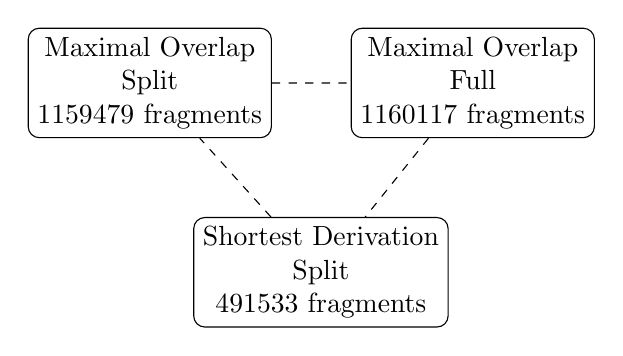
\begin{tikzpicture}[node distance = 1cm]
\node (MOS) [rectangle,rounded corners,draw, align=center]{Maximal Overlap\\ Split\\1159479 fragments};
\node (MOF) [right = of MOS, rectangle,rounded corners,draw, align=center]{Maximal Overlap\\ Full\\1160117 fragments};
\node (SDS) [below right= 1 cm and -1 cm of MOS, rectangle,rounded corners,draw, align=center]{Shortest Derivation\\ Split\\491533 fragments};
\draw[dashed](MOS)--(MOF)--(SDS)--(MOS);
\end{tikzpicture}
\caption{The grammars and their size}
\end{figure}
$p_{unkn}$= $1.41\times 10^{-3}$
\end{frame}

\subsection{Parsing Performance}
\begin{frame}{Scores}
\footnotesize
\begin{table}
%
%\begin{tabular}{l | ccc}
%&Maximal~Overlap&Maximal~Overlap&Shortest~Derivation\\
%&Full& Split&Split\\\hline
%labeled recall&		90,97&	90.14&	84.90\\
%labeled precision&		90.25&	90.10&	84.39\\
%labeled f-measure&		90.61&	90.12&	84.64\\
%exact match&		53.27&	49.53&	39.25\\
%\end{tabular}
%
%\caption{Results for 321 sentences of length$\leq 15$}
%


\begin{tabular}{l | ccc}
&Maximal~Overlap&Maximal~Overlap&Shortest~Derivation\\
& Full& Split&Split\\\hline
labeled recall&		86.17&	85.11&	79.20\\
labeled precision&		86.05&	85.50&	79.32\\
labeled f-measure&		86.11&	85.31&	79.26\\
exact match&		28.32&	25.87&	16.52\\
\end{tabular}

\caption{Results for 1229 sentences of length$\leq 40$}


\end{table}
\end{frame}



\subsection{Analyzing grammars}


\begin{frame}{Split $\leftrightarrow$ Full}
\begin{figure}
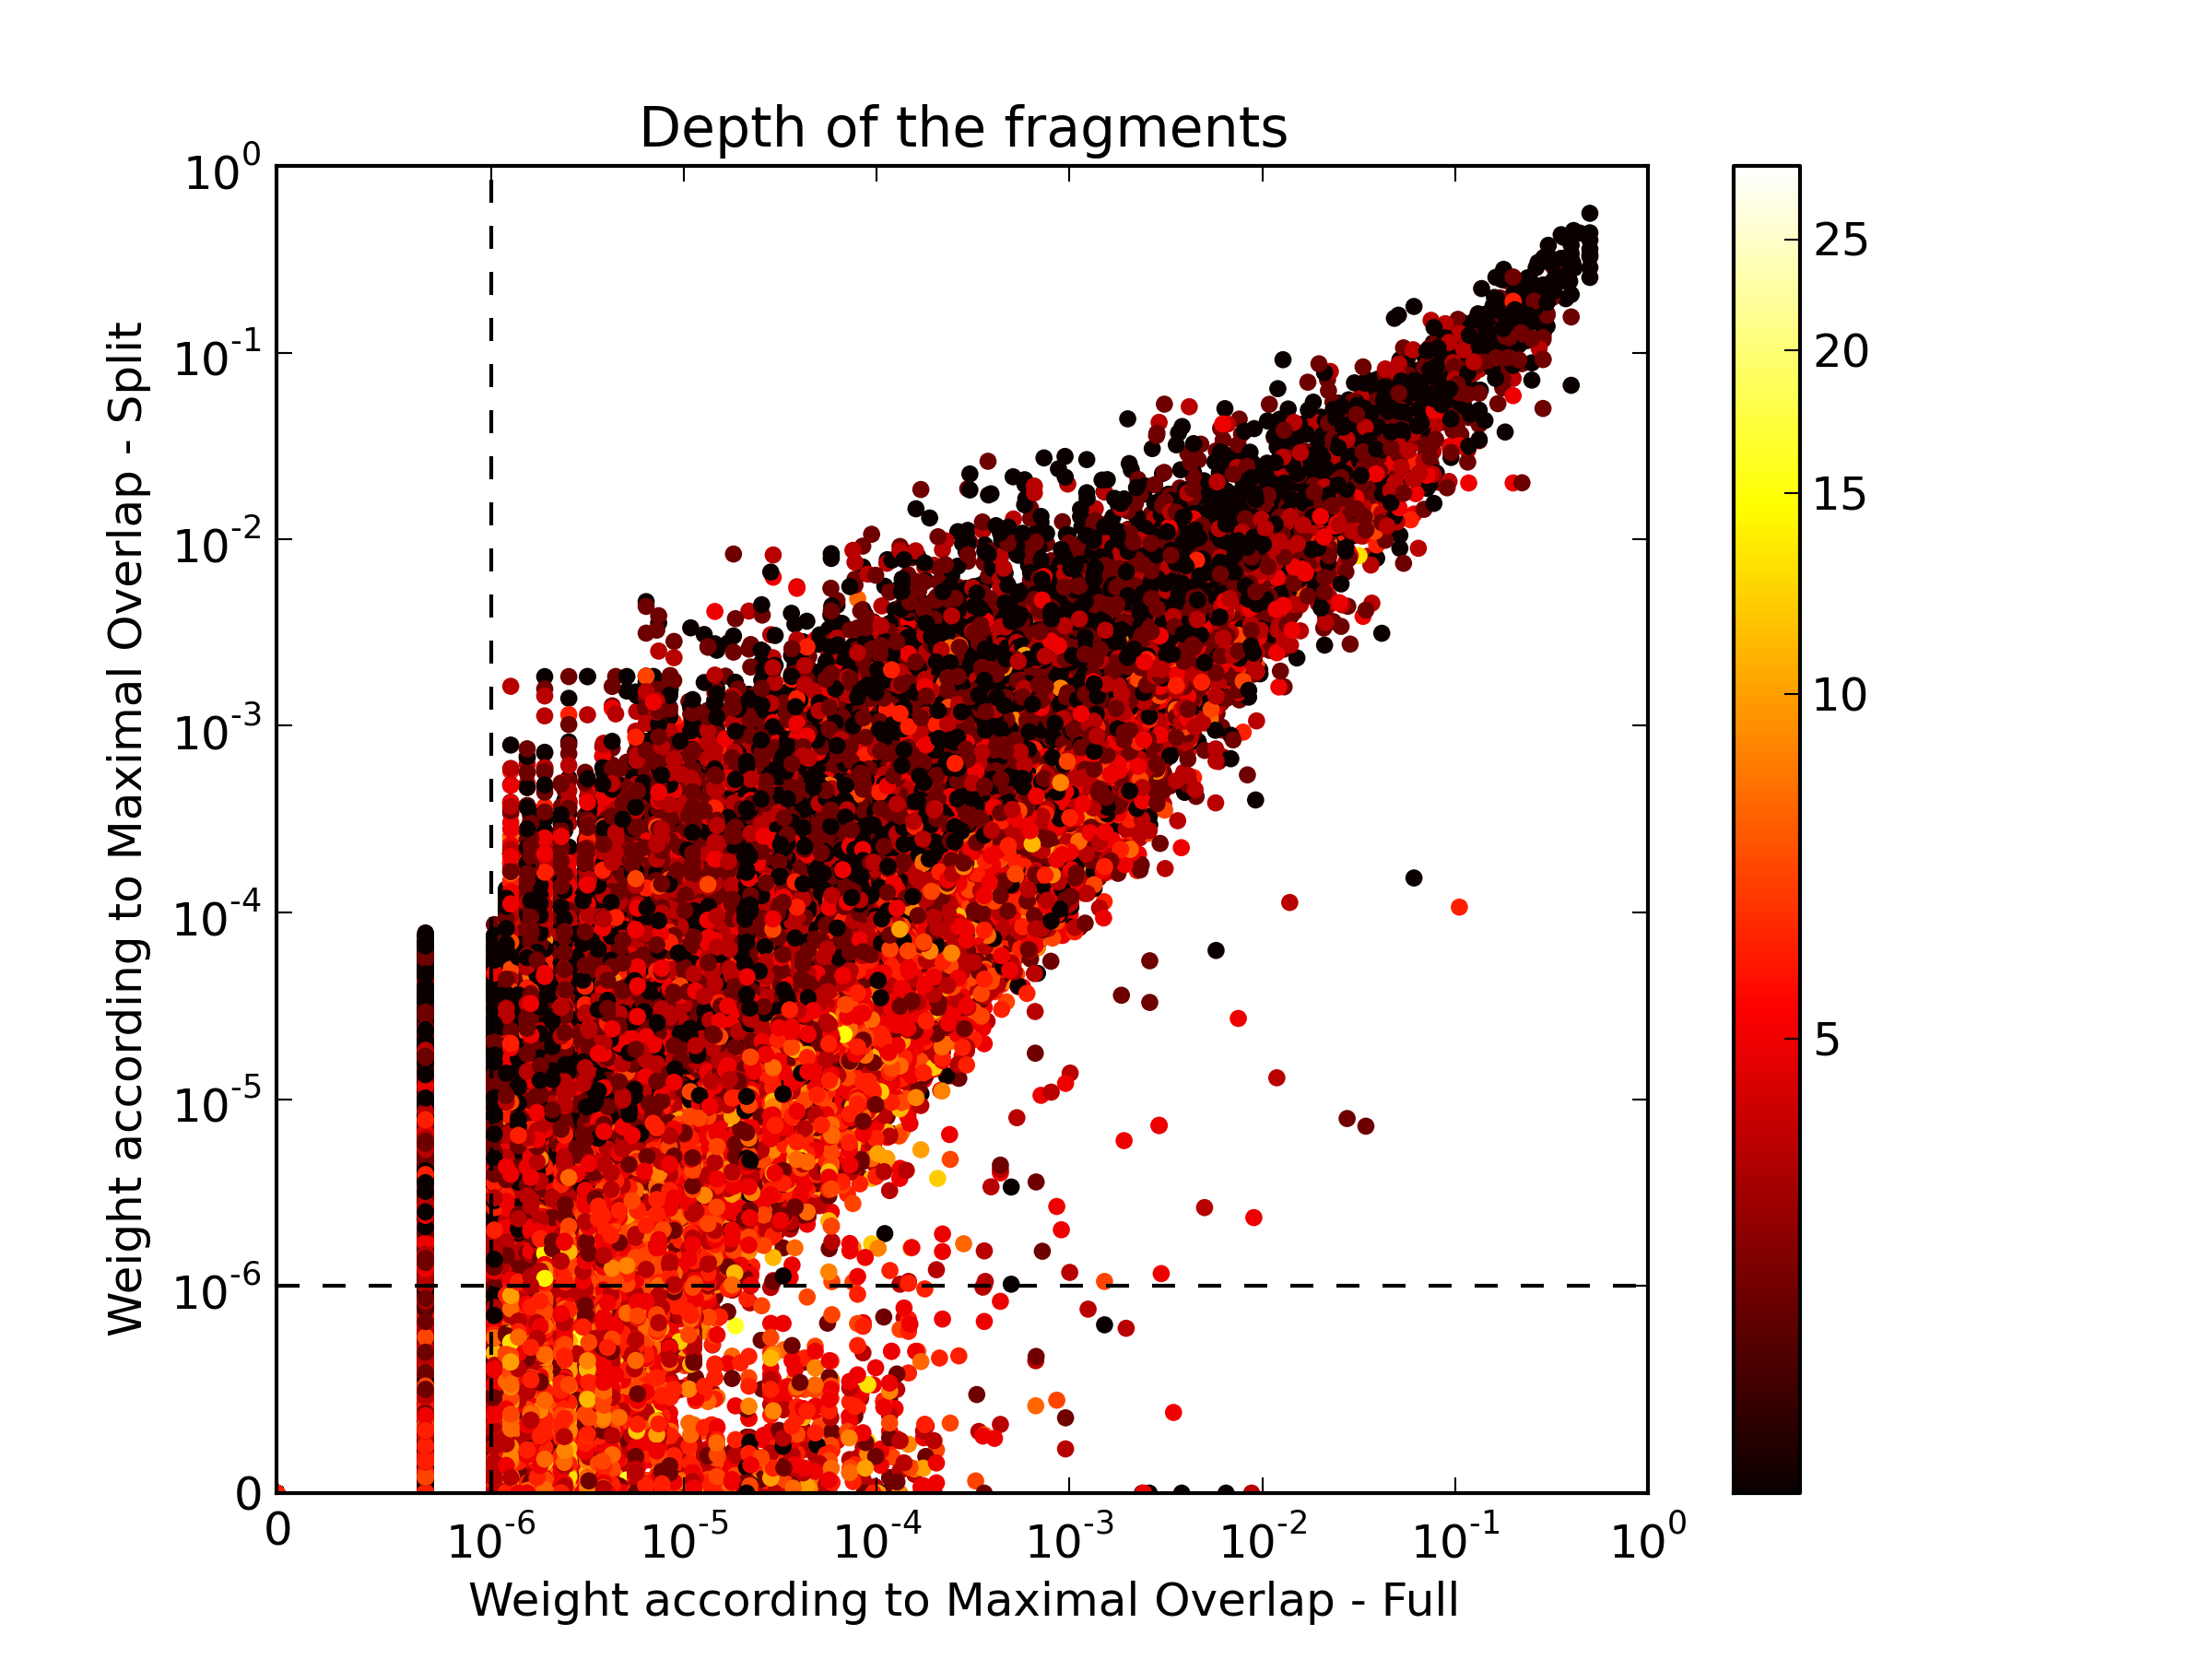
\includegraphics[width=\textwidth,trim=0.5cm 0cm 2.5cm 0.5cm, clip=true]{../data/plots/2.png}
\end{figure}
\end{frame}


\begin{frame}{Maximal overlap $\leftrightarrow$ shortest derivation}

\begin{figure}
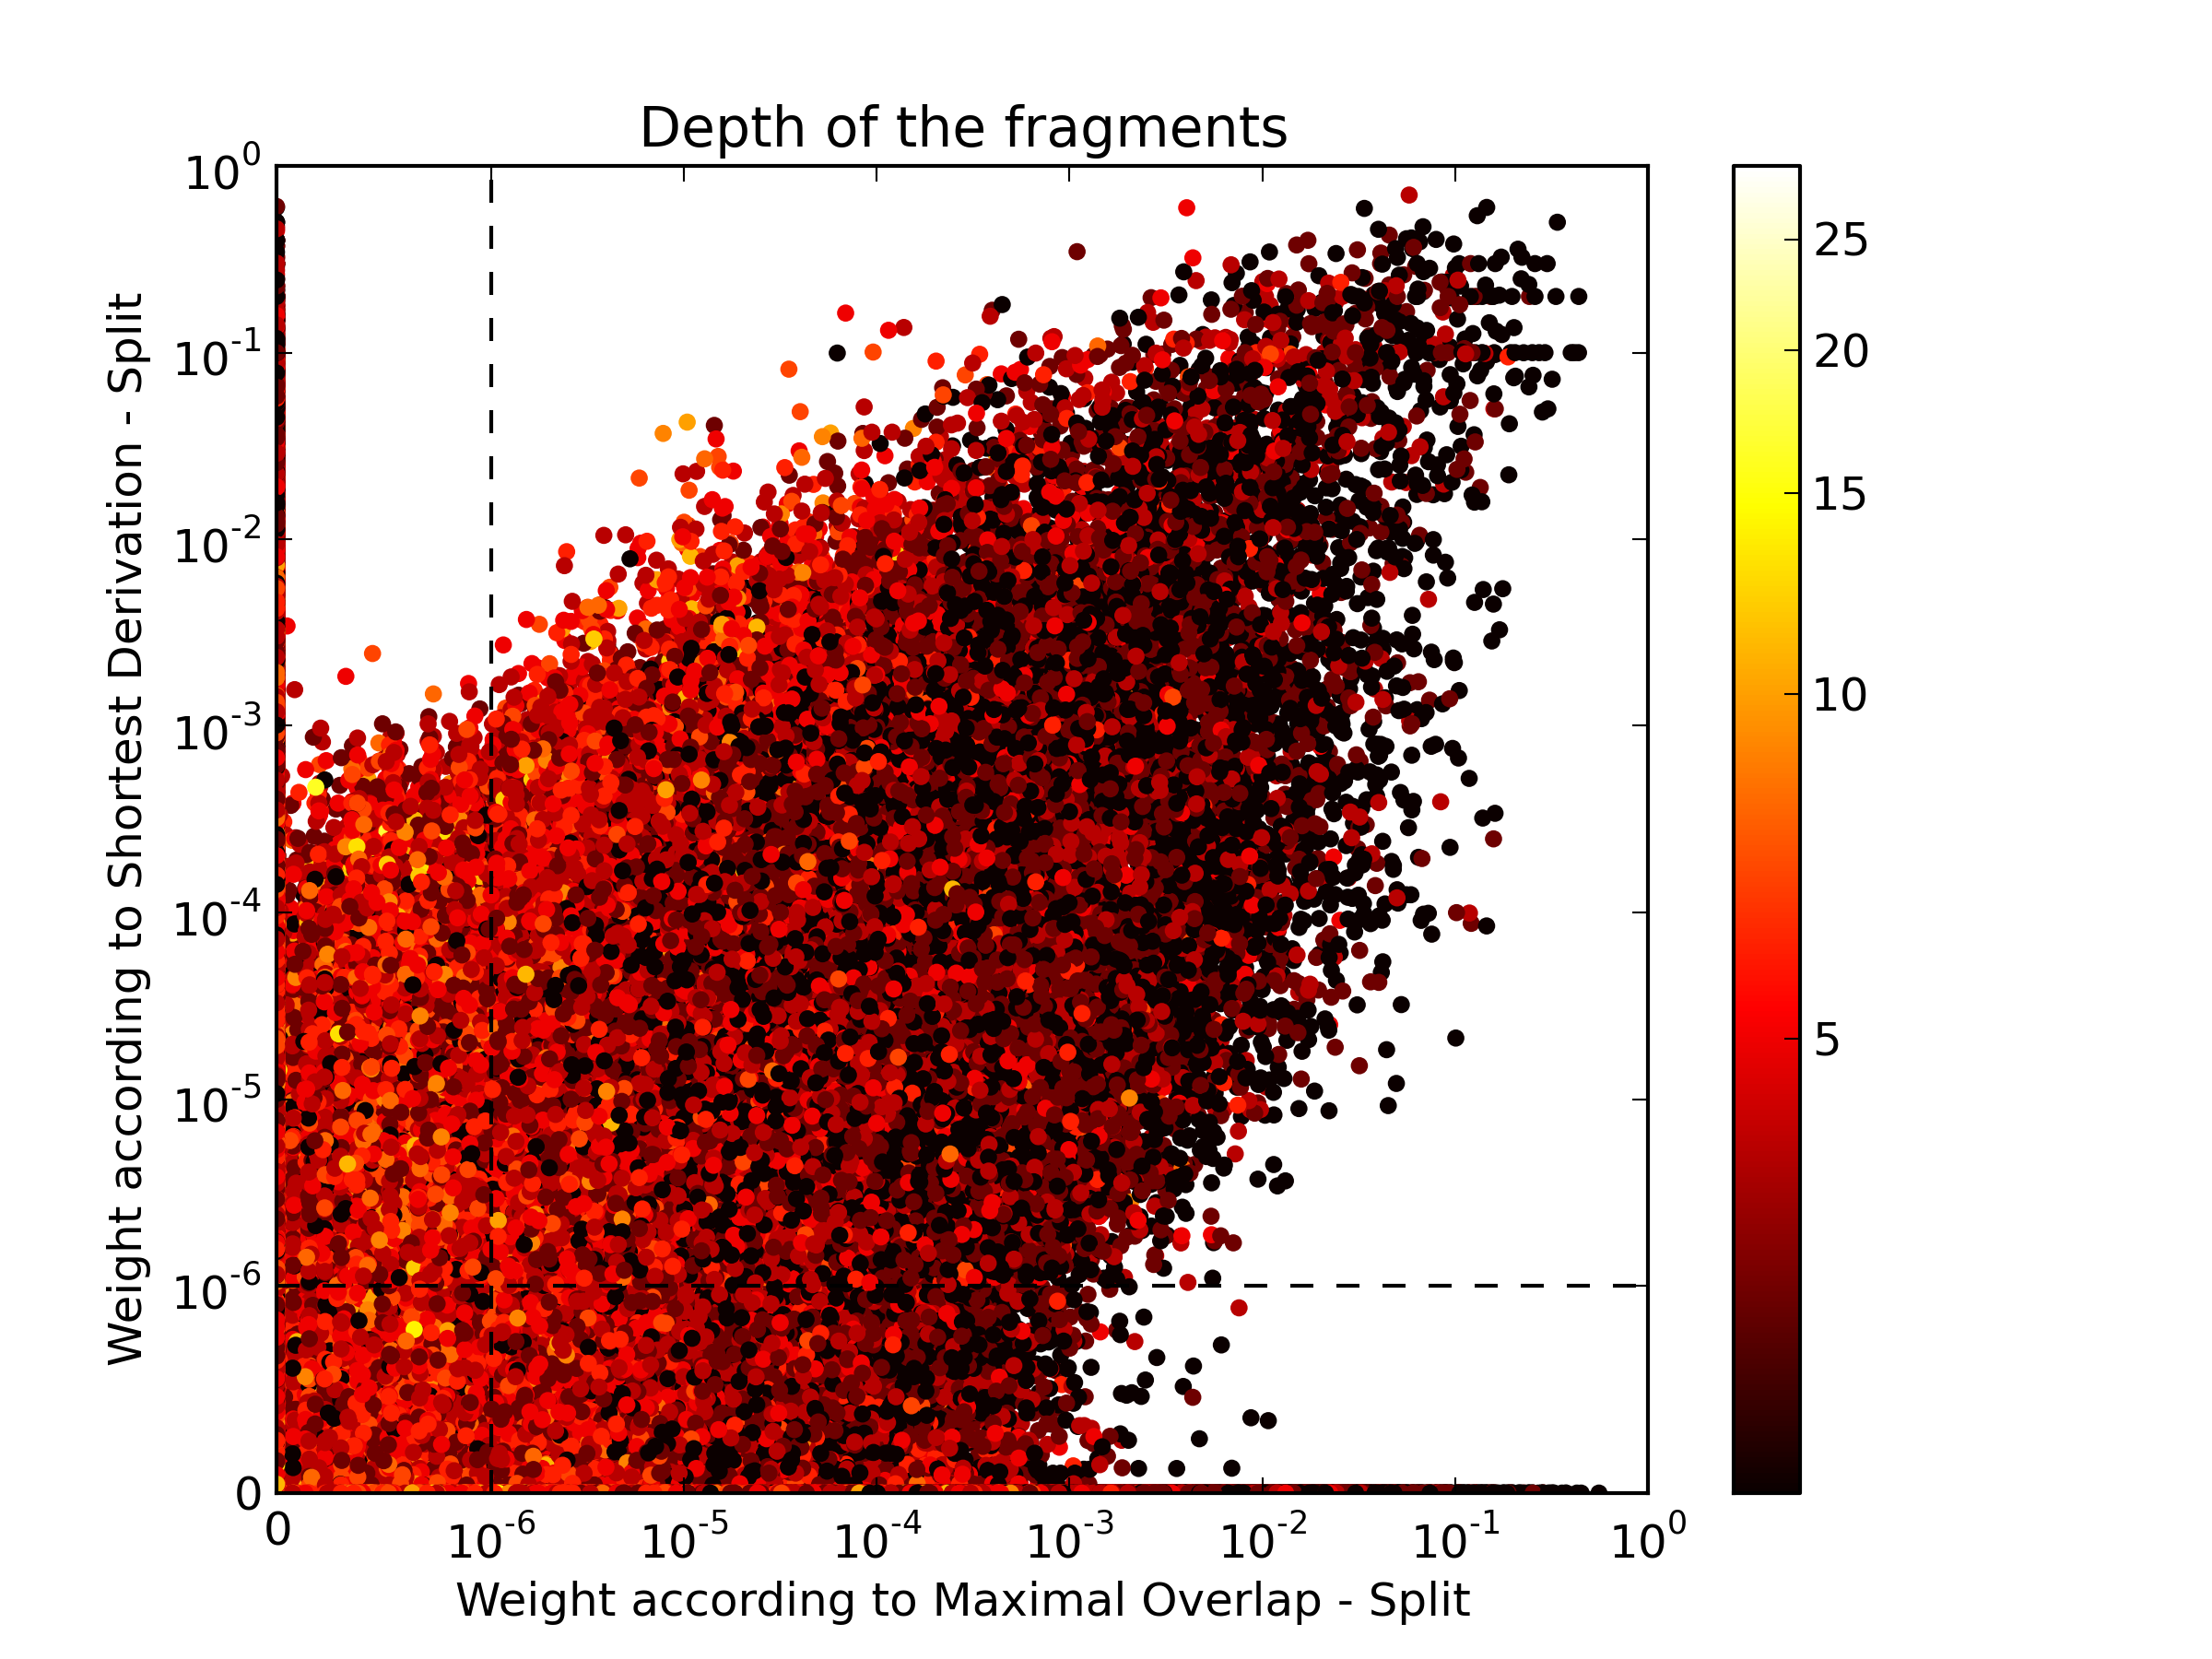
\includegraphics[width=\textwidth,trim=0.5cm 0cm 2.5cm 0.5cm, clip=true]{../data/plots/0.png}
\end{figure}
\end{frame}




\section*{Summary}

\begin{frame}{Summary}

  % Keep the summary *very short*.
  \begin{itemize}
  \item
    \alert{Shortest Derivation} moves weight to larger fragments
  \item
    \alert{Split} moves weight to smaller fragments

  \item
    \alert{Performance} is not necessarily related to \alert{consistency}:   \alert{\dops{}} has bad parsing performance

  \end{itemize}
  
  % The following outlook is optional.
  \vskip0pt plus.5fill
  \begin{itemize}
  \item
    Outlook


    \begin{itemize}
    \item Further analysis %Shortest derivations seem like a good idea, but do not perform good. Why not? 
%Is it just grammar size? Or should we use an estimator other than relative frequency?
\item Other estimators 

%exist. 
%How do their grammars differ? Is there a link between the properties of the grammar and its performance?

    \end{itemize}
  \end{itemize}
\end{frame}

\begin{frame}{Acknowledgments}
\begin{itemize}
\item Andreas van Cranenburgh
\item Khalil Sima'an
\end{itemize}
\end{frame}

\end{document}


